\documentclass[11pt]{article}

\usepackage[utf8]{inputenc}
\usepackage[english]{babel}
\usepackage[T1]{fontenc}
\usepackage{graphicx}
\usepackage[linktocpage=true]{hyperref}
\usepackage[skins]{tcolorbox}
\usepackage{csquotes}
\usepackage{rotating}

\usepackage[
backend=biber,
style=alphabetic,
sorting=ynt
]{biblatex}
\addbibresource{myBibliography.bib}

\usepackage{mathpazo}

\newcommand{\projectName}{Contract Instruction Application}

\begin{document}
\begin{titlepage}
	\newcommand{\HRule}{\rule{\linewidth}{0.5mm}}
    \begin{center}
            
    	\textsc{\LARGE COS 730 - Assignment 1}\\[0.8cm]
    
    	\HRule\\[0.4cm]
    	
    	{\huge\bfseries Contract Instruction Application}\\[0.2cm]
    	
    	{\huge System Requirements Specification}\\[0.2cm]

    	\HRule\\[0.5cm]

	    \textsc{Kyle Gaunt} - u15330967 \\[0cm]
    
    \end{center}
\end{titlepage}

\tableofcontents
\newpage

\section{Introduction}
\begin{center}
\begin{tcolorbox}[skin=widget,
boxrule=1mm,
coltitle=black,
colframe=blue!45!white,
colback=blue!15!white,
width=(.9\linewidth),before=\hfill,after=\hfill,
adjusted title={CONTRACT INSTRUCTION}]
\textit{A written instruction issued by or under the authority of the principal agent to the contractor, which may include drawings and other construction information.}
\tcblower
\cite{ciDefinition}
\end{tcolorbox}
\end{center}
\begin{flushleft}
A Contract Instruction (henceforth CI) has an impact on the various resources of a construction project, be it time, materials or monetary. Due to the importance of the CI in the role of construction, it is vital that construction professionals keep track of and adhere to its contents.\\[0.5cm]

Currently, the process of issuing, editing and interacting with CIs is still done with pen and paper on site, typed up and finalized at the creator's place of work and then distributed using email chains between all involved parties. This means that all relevant information is provided in plain text and must therefore be organised into their relevant categories by each person involved. There is no error checking or notification system to ensure that CIs are being created accurately and alerting users as soon as one is created.\\[0.5cm]

There is a significant space for innovation and a bespoke application that can improve the process from the creation on site all the way through to the distribution of the final document.\\[0.5cm]

In order to solve the aforementioned problems, the \projectName{} has been designed to make the issuing, tracking and closing of CIs as simple and effective as possible. It allows users to send, receive and interact with CIs in real-time and on-the-go, be it in a corporate setting or on an active building site. The project must be accessible on both mobile devices and desktop to cater for all users, be they more office-bound or on-site professionals.\\[0.5cm]

Users can issue a new instruction, specify which areas of the project will be affected, and create custom lists of contacts with which the instruction will be shared. Depending on user privileges, the receiver will be able to interact with the CI accordingly and all relevant parties will be updated in the event of any changes.\\[0.5cm]

The system includes a full reporting suite which will include reports on the project as a whole, as well as user-defined filtered reports on CIs that meet the specified criteria. The reports can be sent out via email to any user(s) specified by the creator of the CI.\\[0.5cm]
\end{flushleft}

\newpage

\section{User Characteristics}
\subsection{Professional}
A Professional in the context of this system refers to a user who will make use of the CI functionalities such as creating, issuing, editing, viewing and accepting CIs. The following assumptions will be made about these users to ensure that the software is designed in a way that suites their needs and expectations:
\begin{itemize}
    \item \textit{Education level:} this type of user can range from an architect or engineer (who require a formal tertiary education) to any sort of contractor (where no formal tertiary education is required). Therefore the minimum education requirement is that of any individual who can read/type.
    \item \textit{Experience:} this user has experience in construction environments and is familiar with the necessary jargon/processes required to operate the application.
    \item \textit{Expertise:} the user will be aware of what a CI is and how the CI process works.
    \item \textit{Technical Skills:} the user is able to operate electronic devices, specifically a mobile device (i.e. smartphone/tablet). Optional experience with a desktop personal computer for those users that require that version of the application.
\end{itemize}
\subsection{Admin}
In addition to all of the functionality offered to Professional users, Administrative users will have the ability to add new users, assign roles to users, allocate and revoke privileges, and monitor the system as a whole. The following assumptions will be made about these users to ensure that the software is designed in a way that suites their needs and expectations:
\begin{itemize}
    \item \textit{Education level:} this type of user requires no formal education to operate the application and so the minimum education requirement is that of any individual who can read/type.
    \item \textit{Experience:} this user has experience in construction environments and is familiar with the necessary jargon/processes required to operate the application. This user also understands the various roles of the Professional users and how they relate to one another.
    \item \textit{Expertise:} the user will be aware of what a CI is and how the CI process works.
    \item \textit{Technical Skills:} the user is able to use electronic devices, specifically a mobile device (i.e. smartphone/tablet). Optional experience with a desktop personal computer for those users that require that version of the application.
\end{itemize}
\newpage

\section{Functional Requirements}
\subsection{R1 - Contract Instruction Operations}
\begin{itemize}
    \item \textit{R1.1 -} System must be able to create a user-defined contract instruction.
    \item \textit{R1.2 -} System must be able to perform various operations on the contract instruction, such as editing and deletion.
    \item \textit{R1.3 -} System must allow for specific contacts to be selected and requests for those users to accept/reject the CI to be sent out.
    \item \textit{R1.4 -} Optional notifications allow users to be notified once changes have been made to the projects with which they are involved.
    \item \textit{R1.5 -} Users must be able to view all CIs that they have been included in.
\end{itemize}
\subsection{R2 - Reporting Suite}
\begin{itemize}
    \item \textit{R2.1 -} Reports must be generated in PDF format.
    \item \textit{R2.2 -} Reports must be created to summarize specific characteristics of the collection of CIs.
    \item \textit{R2.3 -} Reports should be split into two broad categories.
    \begin{itemize}
        \item \textit{R2.3.1 -} Reports can be categorized as those that summarize a specific CI.
        \item \textit{R2.3.2 -} Reports can be categorized as those that summarise the entire project as a whole (all or a specified group of CIs).
    \end{itemize}
\end{itemize}
\subsection{R3 - User Administration}
\begin{itemize}
    \item \textit{R3.1 -} The system must allow for Admin users to create new Contractor users.
    \item \textit{R3.2 -} The system must allow Admin users to assign Contractors to specific projects.
    \item \textit{R3.3 -} The system must allow Admin users to specify/alter a Contractor's role/privileges within a project.
    \item \textit{R3.4 -} The Admin user must be able to specify a list of Contractors that will automatically be included in a CI's communications (Distribution List).
    \item \textit{R3.5 -} The system must allow Admin users to delete Contractors from the system or edit their role within specific projects.
    \item \textit{R3.6 -} The Admin user must NOT be able to edit a Contractors user's profile information beyond their role within a project.
\end{itemize}

\section{Use Cases}
\subsection{U1 - Contract Instruction Process}
    \begin{flushleft}
        \begin{itemize}
            \item The Client creates a CI which will included any relevant professionals (i.e. Contractors).\\[0.5cm]
            \item The Client has the option of adding a notification which will inform all Contractors that the new CI has been created.\\[0.5cm]
            \item If the Client requires the approval of any other Contractors, an approval request can be created.\\[0.5cm]
            \item All users included in the CI will be able to view the CI, additionally, all users included in the acceptance request will be able to accept or deny the request when viewing the CI.\\[0.5cm]
            \item When viewing the CI, the Client has the additional option of editing the CI, which will notify all of the Contractors when a change is made.\\[0.5cm]
            \item Lastly, the Client is able to delete the CI, which will also notify the Contractors.\\[0.5cm]
        \end{itemize}
    \textit{Please see use case diagram \#1 on the next page...}\\[0.5cm]
\end{flushleft}
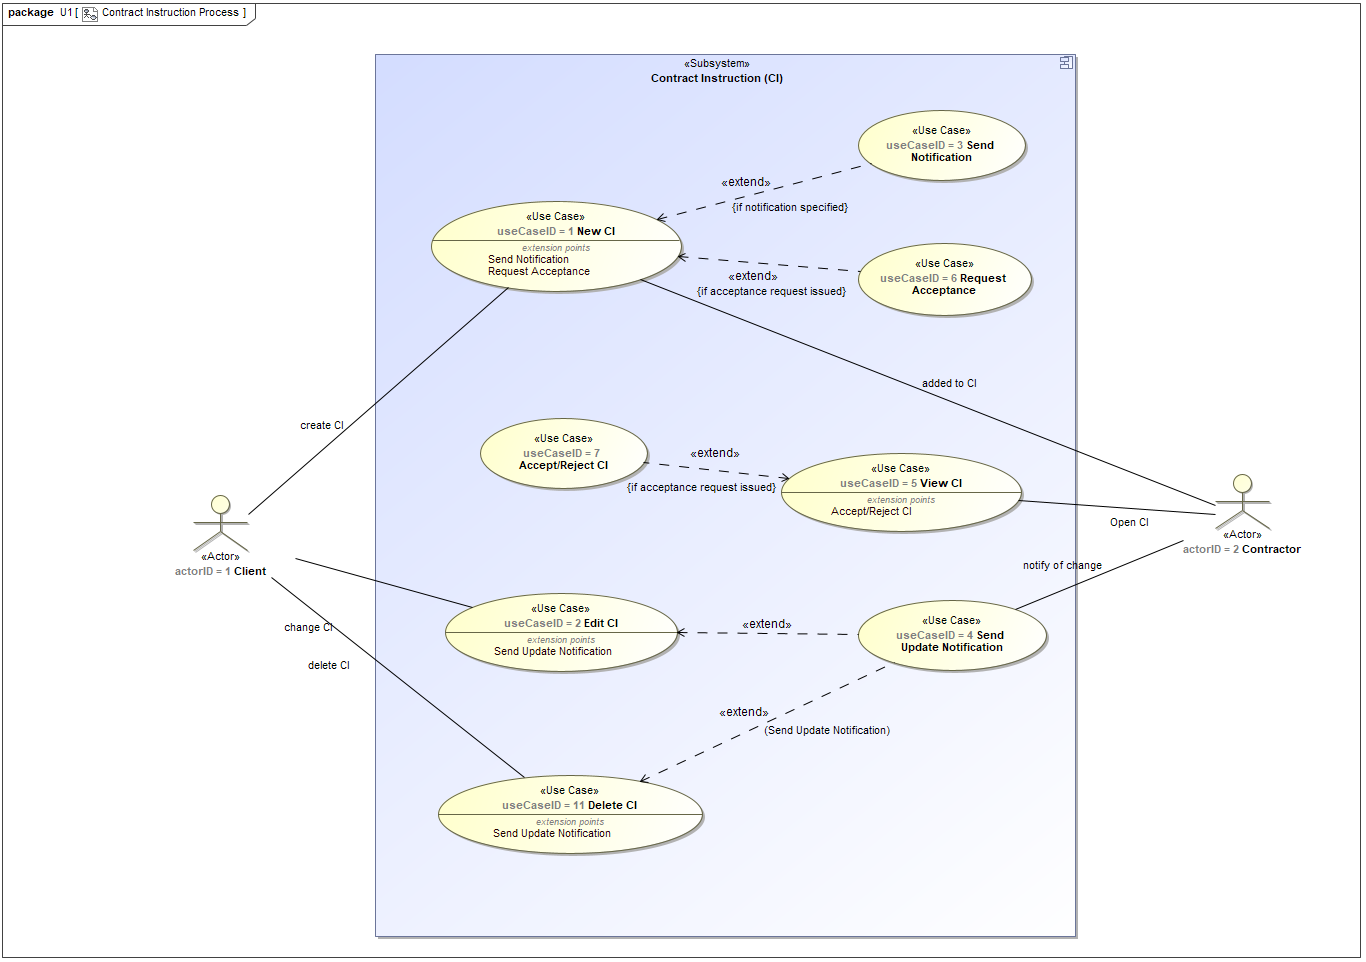
\includegraphics[width = 1.0 \textwidth, height = 1.0 \textwidth]{images/UseCase1.PNG}
\subsection{U2 - Reporting System}
\begin{flushleft}
        \begin{itemize}
            \item The Client can view any CIs created by themselves. The report will include a summary of the specific CI, information about who is included in the CI, the specific roles and responsibilities of each CI member and information about which of those members have/have not yet accepted the CI. \\[0.5cm]
            \item Any reports that the Client has access to can be downloaded from the server.\\[0.5cm]
            \item The Client can send any accessible reports to any of the included members, the contact information of which will be provided by the server.\\[0.5cm]
            \item All information provided to the Reporting system will be fetch from a database on the server.\\[0.5cm]
        \end{itemize}
    \textit{Please see use case diagram \#2...}\\[0.5cm]
\end{flushleft}
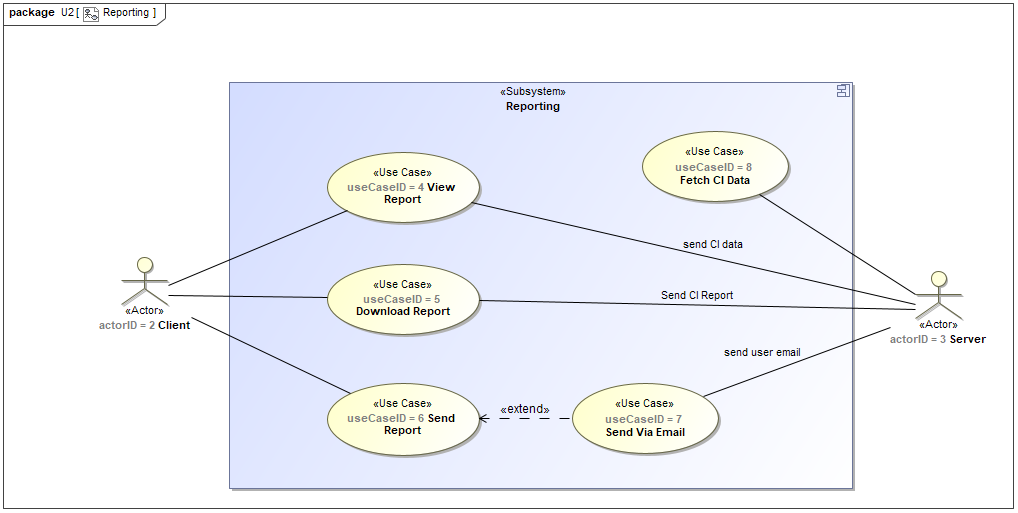
\includegraphics[width = 1.0 \textwidth, height = 0.8 \textwidth]{images/UseCase2.PNG}
\subsection{U3 - Admin User Management}
\begin{flushleft}
        \begin{itemize}
            \item The admin can create a profile for the Contractor.\\[0.5cm]
            \item After the Contractor's account has been created, they can access their profile to edit any personal information settings or can delete their account. Apart from the privileges of each non-admin user, an Admin cannot edit any of a user's profile information.\\[0.5cm]
            \item The Admin can edit each users' privileges within the project in order to ensure that the correct people are performing certain actions within the project. Users will be able to see the extent of their access/editing privileges within their profile but cannot edit their own privileges.\\[0.5cm]
            \item An admin can delete a Contractor's profile.\\[0.5cm]
        \end{itemize}
    \textit{Please see use case diagram \#3...}\\[0.5cm]
\end{flushleft}
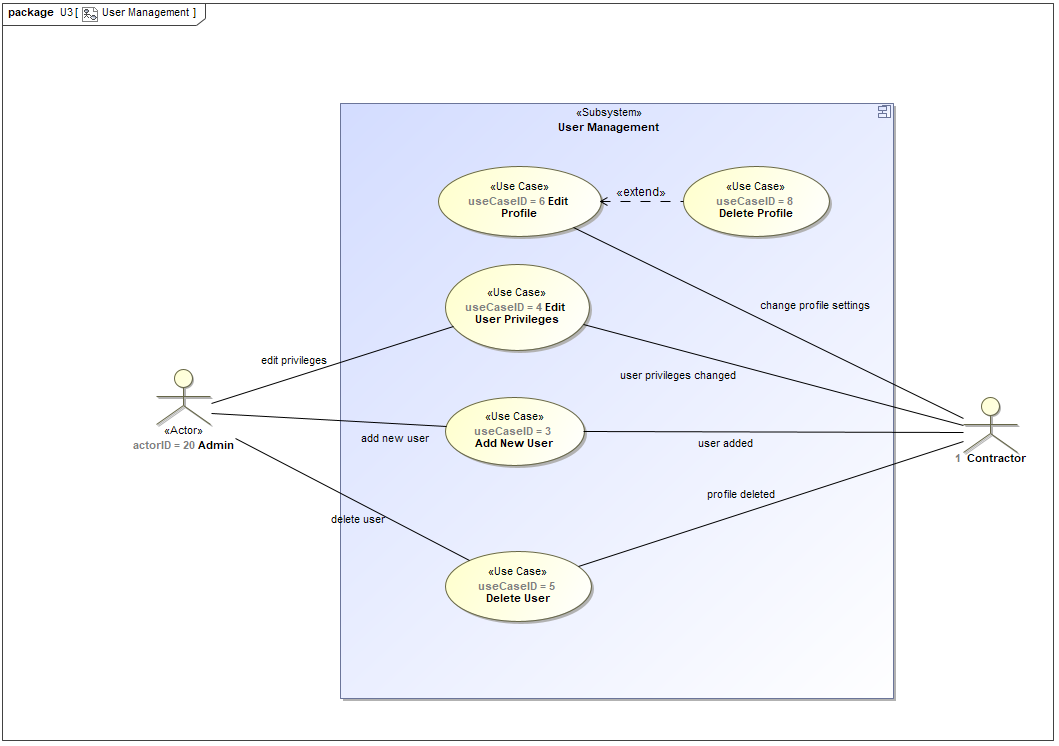
\includegraphics[width = 1.0 \textwidth, height = 0.7 \textwidth]{images/UseCase3.PNG}

 \newpage
\section{Traceability Matrix}
\begin{center}
 \begin{tabular}{||c | c | c | c ||} 
 \hline
  & Contract Instruction Process & Reporting System & Admin User Management \\
 \hline\hline
 R1.1 & X &  &  \\
 \hline
 R1.2 & X &  &  \\
 \hline
 R1.3 & X &  &  \\
 \hline
 R1.4 & X &  &  \\
 \hline
 R1.5 & X &  &  \\
 \hline
 R2.1 &  & X &  \\
 \hline
 R2.2 &  & X &  \\
 \hline
 R2.3 &  & X &  \\
 \hline
 R2.3.1 &  & X &  \\
 \hline
 R2.3.2 &  & X &  \\
 \hline
 R3.1 &  &  & X \\
 \hline
 R3.2 &  &  & X \\
 \hline
 R3.3 &  &  & X \\
 \hline
 R3.4 &  &  & X \\
 \hline
 R3.5 &  &  & X \\
 \hline
 R3.6 &  &  & X \\
 \hline
 QR1.1 & X &  & \\
 \hline
 QR1.2 & X &  & X \\
 \hline
 QR1.3 & X &  & \\
 \hline
 QR2.1 & X & X & X \\
 \hline
 QR3.1 & X & X & X \\
 \hline
 QR3.2 & X & X & X \\
 \hline
 QR4.1 & X & X & X \\
 \hline
 QR4.2 & X & X & X \\
 \hline
 QR5.1 &  &  & X \\
 \hline
 QR5.2 &  &  & X \\
 \hline
 QR5.3 & X &  & X \\
 \hline

\end{tabular}
\end{center}


\section{Non-Functional Requirements}
\subsection{\textit{QR1 -} Availability}
\begin{itemize}
    \item \textit{QR1.1 -} The system has to have high availability to handle user operations in real-time due to the urgent nature of the processes and procedures involved.
    \item \textit{QR1.2 -} The system should be available at least 99 percent of the time, apart from where network errors are involved.
    \item \textit{QR1.3 -} The system should be able to operate without an active Internet connection as most active construction sites do not always have Internet access freely available.
\end{itemize}

\subsection{\textit{QR2 -} Performance}
\begin{itemize}
    \item \textit{QR2.1 -} The system must perform its operations in a manner that is swift, efficient and accurate to ensure that any changes made are done so as instantaneously as possible, with minimum strain on the system and with no concern regarding authenticity and integrity.
\end{itemize}

\subsection{\textit{QR3 -} Scalability}
\begin{itemize}
    \item \textit{QR3.1 -} The system should be able to scalable in order to accommodate additional/growing user operations, especially during peak work hours. Off-peak hour reduction of resources would be an advantageous feature for the system.
    \item \textit{QR3.2 -} The system will be deployed on an automatic scaling infrastructure such as Docker, in conjunction with Kubernetes in order to allow for efficient and easy scaling, as well as state recovery should the application crash. More resources can be allocated to the system dynamically as needed.
\end{itemize}

\subsection{\textit{QR4 -} Maintainability}
\begin{itemize}
    \item \textit{QR4.1 -} The system structure will be modular to adhere to the concept of low coupling and high cohesion. This would help its maintainability because when updating a specific module within the system, the changes remain localized instead of promulgating changes everywhere throughout the system. Once the changes have been made and tested, they can be seamlessly integrated into the live system.
    \item \textit{QR4.2 -} A coding standards document will be included to ensure that all parties follow the same coding procedures and protocols. This will make the system easier to understand and increase the ability for multiple parties to operate on the project in conjunction with one another.
\end{itemize}

\subsection{\textit{QR5 -} Security}
\begin{itemize}
    \item \textit{QR5.1 -} Secure login will be required for all users. This will be done by means of a third-party security application such as OAuth.
    \item \textit{QR5.2 -} A secure login system will be implemented and private user information would have to be secured i.e information that would used for authentication purposes like email addresses.
    \item \textit{QR5.3 -} Information regarding the projects and the information associated with them will also need to be secured to prevent any potential breach of Intellectual Property or Trade Secret laws being broken.

\end{itemize}

\newpage
\section{Domain Model}
\begin{flushleft}
The domain model below is used to describe the main components of the system. Please note:\\[0.5cm]
\begin{itemize}
    \item A user can be assigned to multiple CIs.
    \item A CI can have multiple users.
    \item A CI can contain multiple files but can also not contain any.
    \item A CI can only belong to one project.
    \item A project can have multiple CIs.
    \item A project can have multiple users.
    \item A user can be assigned to multiple projects but can only be assigned to an individual project once.
    \item A file can only belong to one CI.
    \item A user can only belong to one company.
    \item A company can have multiple users.
    \item A project can only have one distribution list.
    \item A distribution list can only be assigned to one project, but can be assigned to multiple CIs.
    \item A project report can only belong to one project, but multiple reports can be generated for that project.
    \item A CI report can only belong to one project, but multiple reports can be generated for that project.

\end{itemize}


\textit{Please see diagram below.}\\[0.5cm]
\end{flushleft}
\begin{sidewaysfigure}
    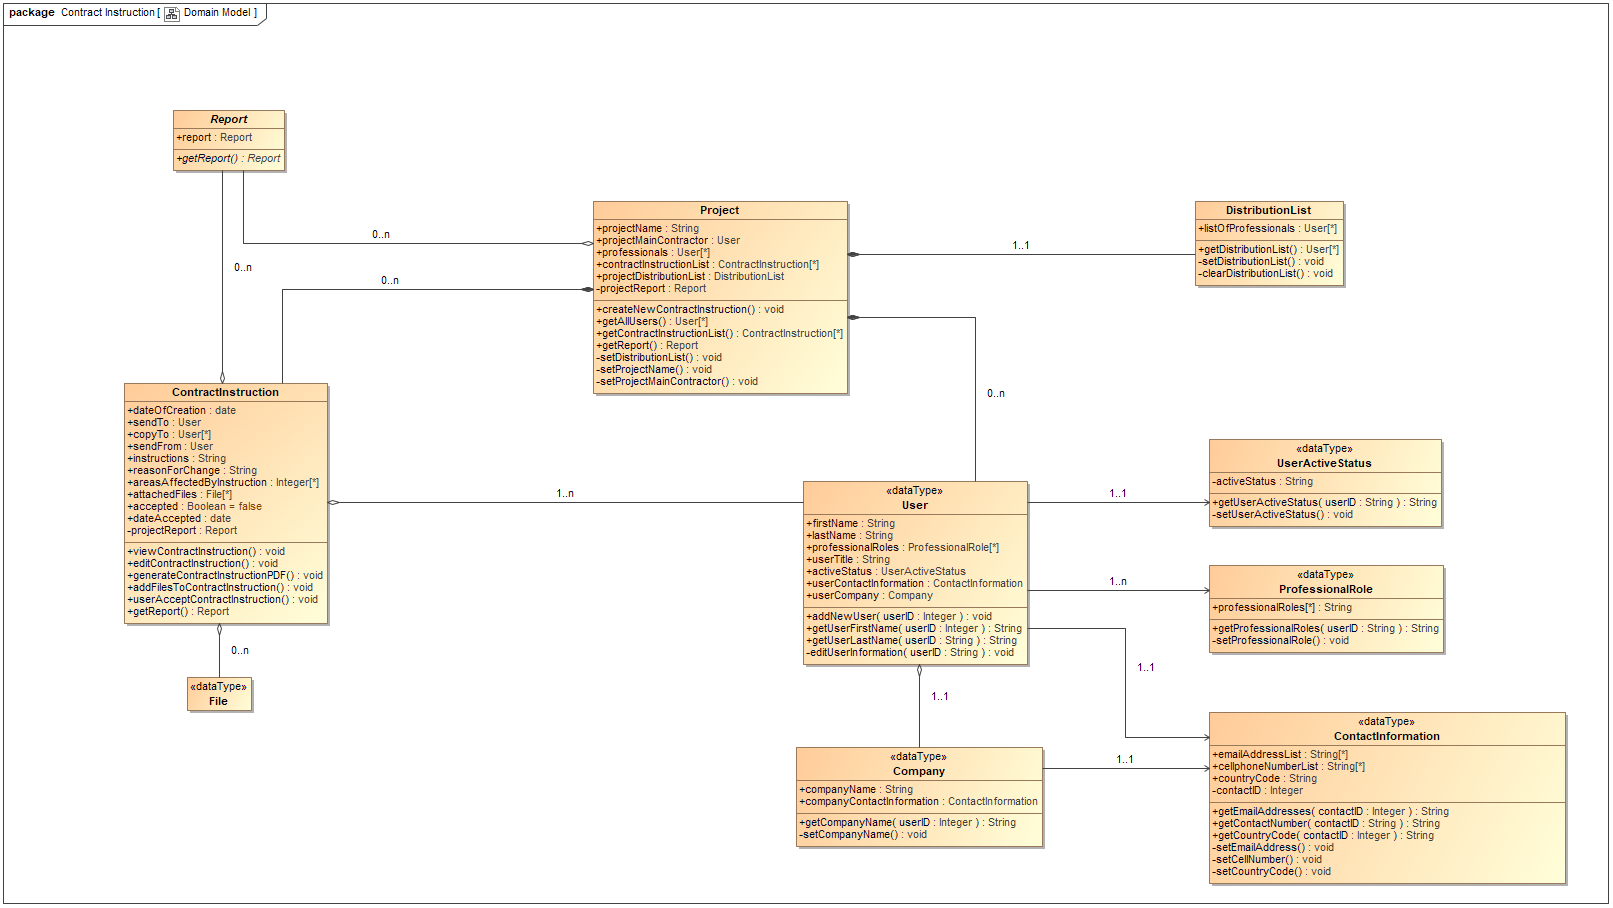
\includegraphics[width = 1.0 \textwidth, height = 0.6 \textwidth]{images/DomainModel.PNG}
\end{sidewaysfigure}
 \newpage

\end{document}
